\documentclass[11pt,a4paper]{article}
\usepackage{estilo-libro}
\usetikzlibrary{matrix,backgrounds}
\usepackage{needspace}
% Que un título de paso no quede solo al final de una página
\let\pasobase\paso
\renewcommand{\paso}[1]{\needspace{7\baselineskip}\pasobase{#1}}

% ---------- Tablas húngaras en TikZ ----------
% Fila 1 = encabezados, columna 1 = nombres. Los datos van desde la celda (2,2).
\tikzset{
  htab/.style={matrix of nodes, ampersand replacement=\&, row sep=0pt, column sep=0pt,
    nodes={text width=#1, align=center, minimum height=6.4mm, inner sep=1.5pt, font=\small, anchor=center},
    column 1/.style={nodes={text width=21mm, font=\small\bfseries}},
    row 1/.style={nodes={font=\footnotesize\bfseries}}},
  htab/.default=10.5mm,
  nota col/.style={column #1/.style={nodes={text width=16mm, font=\footnotesize\itshape}}},
  tapa/.style={line width=3pt, gray!60, line cap=round},
  tab9/.style={htab=12mm, column 1/.style={nodes={text width=24mm, font=\small\bfseries}}, row 1/.style={nodes={font=\scriptsize\bfseries}}},
  mini/.style={htab=7mm, column 1/.style={nodes={text width=11mm, font=\small\bfseries}}},
  asignado/.style={draw, circle, thick, minimum size=5.6mm, inner sep=0pt},
}
% \rejilla{nombre}{última fila}{última columna}
\newcommand{\rejilla}[3]{%
  \foreach \i in {2,...,#2}{\foreach \j in {2,...,#3}{%
    \draw[gray!55, thin] (#1-\i-\j.north west) rectangle (#1-\i-\j.south east);}}%
  \draw[thick] (#1-2-2.north west) rectangle (#1-#2-#3.south east);}
% Fila o columna ficticia sombreada (debajo de los números)
\newcommand{\sfila}[3]{\begin{pgfonlayer}{background}\fill[gray!16] (#1-#2-2.north west) rectangle (#1-#2-#3.south east);\end{pgfonlayer}}
\newcommand{\scol}[3]{\begin{pgfonlayer}{background}\fill[gray!16] (#1-2-#2.north west) rectangle (#1-#3-#2.south east);\end{pgfonlayer}}
% Líneas que tapan ceros: \lfila{nombre}{fila}{última columna}, \lcol{nombre}{columna}{última fila}
\newcommand{\lfila}[3]{\begin{pgfonlayer}{background}\draw[tapa] ($(#1-#2-2.west)+(-1.5pt,0)$) -- ($(#1-#2-#3.east)+(1.5pt,0)$);\end{pgfonlayer}}
\newcommand{\lcol}[3]{\begin{pgfonlayer}{background}\draw[tapa] ($(#1-2-#2.north)+(0,1.5pt)$) -- ($(#1-#3-#2.south)+(0,-1.5pt)$);\end{pgfonlayer}}
% Cero asignado: \cero{nombre}{fila-columna}
\newcommand{\cero}[2]{\node[asignado] at (#1-#2) {};}
% Texto al pie de una tabla: \pie{nombre}{última fila}{última columna}{texto}
\newcommand{\pie}[4]{\node[font=\footnotesize, below=1mm, align=center] at ($(#1-#2-2.south west)!0.5!(#1-#2-#3.south east)$) {#4};}
\newcommand{\linea}{\tikz[baseline=-0.6ex]\draw[tapa] (0,0)--(0.6,0);}
\newcommand{\cajaM}{\textbf{M}}

\title{\textbf{Casos particulares del problema de asignación}\\[4pt]\large Explicación de cada caso y ejercicios resueltos}
\author{Investigación de Operaciones · Asignación y flujo en redes}
\date{}

\begin{document}
\maketitle
\tableofcontents
\newpage

% =====================================================================
\part{¿En qué consisten los casos particulares?}

\section{¿Qué tipo de problema resuelve?}

El \textbf{problema de asignación} consiste en repartir \textbf{tareas} entre \textbf{agentes} (personas,
máquinas, plantas) de modo que cada agente haga una tarea, cada tarea la haga un agente y el
\textbf{costo total sea el menor posible}. Los datos se ponen en una tabla: cada fila es un agente, cada
columna es una tarea y cada casilla dice cuánto cuesta que ese agente haga esa tarea.

El método de Kuhn-Munkres, más conocido como \textbf{método húngaro}, resuelve este problema a mano con
unas pocas restas. Pero solo sabe trabajar con una tabla ``perfecta'': \textbf{cuadrada} (tantos agentes como
tareas), de \textbf{costos} que se quieren \textbf{minimizar} y en la que \textbf{cualquier} agente puede hacer
\textbf{cualquier} tarea. En la vida real casi nunca es así:

\begin{ojo}
Tres amigos comparten un departamento y hay \textbf{cuatro} tareas: cocinar, lavar, barrer y hacer las compras.
Cada uno tarda un tiempo distinto en cada tarea. Pero ocurre que:
\begin{itemize}[itemsep=1pt, topsep=2pt]
  \item hay \textbf{más tareas que personas} (si cada uno hace una sola, una tarea se quedará sin hacer);
  \item Luis \textbf{no puede} hacer las compras porque no tiene auto;
  \item Ana es tan rápida que \textbf{puede hacer dos tareas};
  \item y si en vez de tiempos tuviéramos \textbf{puntos de gusto} (cuánto le agrada a cada uno cada tarea),
        querríamos \textbf{el máximo}, no el mínimo.
\end{itemize}
Cada una de estas situaciones es un \textbf{caso particular} del problema de asignación.
\end{ojo}

La buena noticia es que \textbf{no hace falta un método nuevo para cada caso}. Basta con ``arreglar'' la tabla
antes de empezar, para que quede con la forma que el método húngaro entiende. Después se aplica el método
de siempre y, al final, se traduce el resultado al problema real.

% =====================================================================
\section{La idea: preparar la tabla y usar el método de siempre}

Todos los casos particulares siguen el mismo camino: se hace una pequeña transformación a la tabla, se resuelve
con el método húngaro y se interpreta la respuesta.

\begin{center}
\begin{tikzpicture}[node distance=5mm, >=Stealth,
  caja/.style={draw, rounded corners=2pt, fill=gray!8, align=center, text width=2.45cm, inner sep=4pt, font=\small},
  fuerte/.style={caja, fill=gray!25, font=\small\bfseries}]
  \node[caja] (real) {Problema real\\ \footnotesize (no cuadrado, de máximo, con prohibiciones\dots)};
  \node[fuerte, right=of real] (prep) {Preparar la tabla};
  \node[caja, right=of prep] (std) {Tabla cuadrada de costos a minimizar};
  \node[fuerte, right=of std] (hung) {Método húngaro};
  \node[caja, right=of hung] (trad) {Traducir: quitar lo ficticio y sumar los valores originales};
  \draw[->, thick] (real) -- (prep);
  \draw[->, thick] (prep) -- (std);
  \draw[->, thick] (std) -- (hung);
  \draw[->, thick] (hung) -- (trad);
\end{tikzpicture}
\end{center}

\needspace{9\baselineskip}
Las transformaciones son cuatro, y cada una tiene una idea muy simple detrás:

\begin{center}\small
\begin{tabular}{p{3.6cm}p{5.0cm}p{6.6cm}}
\toprule
\textbf{Situación} & \textbf{Arreglo} & \textbf{Por qué funciona} \\
\midrule
Faltan agentes o tareas & Agregar \textbf{ficticios} con costo 0 & Lo ficticio no cuesta nada: es ``quedarse sin pareja''. \\
Se quiere el máximo & Restar cada valor del \textbf{mayor} de la tabla & Se minimiza ``lo que se deja de ganar''. \\
Una pareja es imposible & Poner un costo $M$ gigantesco & Nadie elige algo carísimo si tiene otra opción. \\
Un agente hace varias tareas & \textbf{Copiar} su fila una vez por tarea & Cada copia es ``un turno'' del mismo agente. \\
\bottomrule
\end{tabular}
\end{center}

Hay además un quinto caso que no se prepara, sino que \textbf{aparece al final}: los \textbf{óptimos múltiples},
cuando hay más de una forma de asignar con el mismo costo mínimo.

% =====================================================================
\section{Repaso del método húngaro}\label{sec:repaso}

Recordamos en una página cómo funciona el método, con tres personas, tres tareas y los minutos que tarda cada una.

\begin{center}
\begin{tikzpicture}
\matrix (r0) [htab=7mm, column 1/.style={nodes={text width=10mm, font=\small\bfseries}}] {
 \& T1 \& T2 \& T3 \\
Ana  \& 9 \& 2 \& 7 \\
Beto \& 6 \& 4 \& 3 \\
Caro \& 5 \& 8 \& 1 \\
};
\rejilla{r0}{4}{4}
\pie{r0}{4}{4}{costos originales}
\end{tikzpicture}\qquad
\begin{tikzpicture}
\matrix (r1) [htab=7mm, column 1/.style={nodes={text width=10mm, font=\small\bfseries}}] {
 \& T1 \& T2 \& T3 \\
Ana  \& 7 \& 0 \& 5 \\
Beto \& 3 \& 1 \& 0 \\
Caro \& 4 \& 7 \& 0 \\
};
\rejilla{r1}{4}{4}
\pie{r1}{4}{4}{paso 1}
\end{tikzpicture}\qquad
\begin{tikzpicture}
\matrix (r2) [htab=7mm, column 1/.style={nodes={text width=10mm, font=\small\bfseries}}] {
 \& T1 \& T2 \& T3 \\
Ana  \& 4 \& 0 \& 5 \\
Beto \& 0 \& 1 \& 0 \\
Caro \& 1 \& 7 \& 0 \\
};
\rejilla{r2}{4}{4}
\cero{r2}{2-3}\cero{r2}{3-2}\cero{r2}{4-4}
\pie{r2}{4}{4}{pasos 2 a 5}
\end{tikzpicture}
\end{center}

\begin{enumerate}[leftmargin=*, itemsep=3pt, label=\textbf{Paso \arabic*.}]
  \item \textbf{Restar el menor de cada fila} (aquí 2, 3 y 1). Cada fila queda con al menos un cero. No cambia cuál
        es la mejor asignación: a esa persona le toca \emph{alguna} tarea, así que ese costo lo paga sí o sí.
  \item \textbf{Restar el menor de cada columna} (aquí 3, 0 y 0). Un cero quiere decir ``esta pareja es de las más baratas''.
  \item \textbf{Tapar los ceros con el menor número de líneas} que recorren filas o columnas completas. Si hacen
        falta tantas líneas como filas, ya se puede asignar. Aquí hacen falta 3: se pasa al paso 5.
  \item \textbf{Si faltan líneas, ajustar con $k$}, el menor número \textbf{sin ninguna línea}: se le resta $k$ a lo
        no tapado y se le suma $k$ a los \textbf{cruces de dos líneas}. Aparece un cero nuevo y se vuelve al paso 3.
        (El ejercicio 2 de la Parte II tiene un ajuste completo.)
  \item \textbf{Asignar} un cero por fila y por columna, empezando por las filas o columnas con \textbf{un solo cero},
        y encerrarlos en un círculo. Aquí: Ana $\to$ T2, Beto $\to$ T1 y Caro $\to$ T3. El costo se calcula con la
        \textbf{tabla original}: $2 + 6 + 1 = 9$ minutos.
\end{enumerate}

% =====================================================================
\section{Las palabras que se usan}

\begin{center}\small
\begin{tabular}{p{2.9cm}p{12.6cm}}
\toprule
\textbf{Término} & \textbf{Qué significa} \\
\midrule
Agente y tarea & Quien hace el trabajo es una \textbf{fila}; lo que hay que hacer es una \textbf{columna}. Cada casilla es un costo. \\
Balanceado & Que hay tantos agentes como tareas: la tabla es cuadrada. \\
Ficticio & Fila o columna que \textbf{no existe}, con costo 0, agregada para cuadrar la tabla. Lo que le toque queda sin pareja. \\
$M$ & Un número tan grande como haga falta. Se pone en las parejas \textbf{prohibidas}. \\
Pérdida & ``Pérdida de oportunidad'': lo que se deja de ganar al elegir una pareja en lugar de la mejor de la tabla. \\
Línea & Raya que tapa una fila o una columna completa. Aquí se dibuja así: \linea. \\
$k$ & El menor de los números que quedan sin tapar. Sirve para crear ceros nuevos. \\
Cero asignado & El cero que se escoge para formar una pareja. Se encierra en un círculo: \asg{0}. \\
Óptimos múltiples & Dos o más asignaciones distintas con el mismo costo mínimo. \\
Infactible & Que no hay forma de asignar a todos sin usar una pareja prohibida. \\
\bottomrule
\end{tabular}
\end{center}

% =====================================================================
\section{Los casos particulares, uno por uno}\label{sec:casos}

En cada caso se da la receta y un ejemplo pequeño. En las tablas, lo \textbf{sombreado} es ficticio.

\paso{Caso 1. Problema no balanceado: agregar filas o columnas ficticias}
Si hay \textbf{menos agentes que tareas}, se agregan filas ficticias; si hay \textbf{menos tareas que agentes},
se agregan columnas ficticias. Se agregan las que falten para que la tabla quede cuadrada, y todas sus casillas
valen \textbf{0}.

\begin{minipage}[c]{0.36\textwidth}
\centering
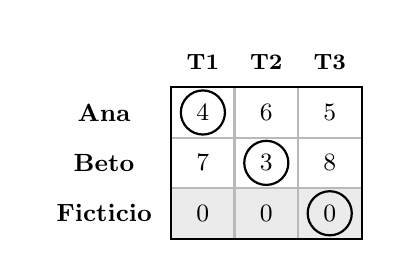
\begin{tikzpicture}
\matrix (c1) [mini, column 1/.style={nodes={text width=16mm, font=\small\bfseries}}] {
 \& T1 \& T2 \& T3 \\
Ana  \& 4 \& 6 \& 5 \\
Beto \& 7 \& 3 \& 8 \\
Ficticio \& 0 \& 0 \& 0 \\
};
\sfila{c1}{4}{4}
\rejilla{c1}{4}{4}
\cero{c1}{2-2}\cero{c1}{3-3}\cero{c1}{4-4}
\end{tikzpicture}
\end{minipage}\hfill
\begin{minipage}[c]{0.62\textwidth}
\textit{Ejemplo:} dos personas y tres tareas. Se agrega un trabajador ficticio con costos 0. Al resolver,
Ana hace T1 y Beto hace T2 (los círculos marcan el resultado final). El ficticio queda con T3: eso quiere decir
que \textbf{T3 no la hace nadie}. El costo real es $4 + 3 = 7$; el 0 del ficticio no se suma.
\end{minipage}

\medskip
El costo 0 es justo: dejar una tarea sin hacer no cuesta nada \emph{dentro del modelo}. Si dejarla sin hacer sí
tuviera un costo (una multa, un cliente perdido), se pone ese valor en la fila ficticia en lugar de 0.

\paso{Caso 2. Maximización: restar cada valor del mayor}
Si los números son \textbf{ganancias} y se quiere el máximo, se busca el \textbf{mayor número de toda la tabla}
y se calcula, para cada casilla,
\[
\text{pérdida} = \text{mayor} - \text{valor}.
\]
La nueva tabla dice \textbf{cuánto se deja de ganar} en cada pareja. Minimizar lo que se deja de ganar es lo
mismo que ganar lo máximo, así que esa tabla se resuelve con el método húngaro normal. (Otra forma equivalente
es multiplicar todos los valores por $-1$; se usa menos a mano porque aparecen negativos.)

\begin{minipage}[c]{0.52\textwidth}
\centering
\begin{tikzpicture}
\matrix (c2) [mini] {
 \& T1 \& T2 \& T3 \\
Ana  \& 8 \& 6 \& 3 \\
Beto \& 5 \& 9 \& 4 \\
Caro \& 7 \& 2 \& 6 \\
};
\rejilla{c2}{4}{4}
\pie{c2}{4}{4}{ganancias}
\end{tikzpicture}\quad
\begin{tikzpicture}
\matrix (c2b) [mini] {
 \& T1 \& T2 \& T3 \\
Ana  \& 1 \& 3 \& 6 \\
Beto \& 4 \& 0 \& 5 \\
Caro \& 2 \& 7 \& 3 \\
};
\rejilla{c2b}{4}{4}
\pie{c2b}{4}{4}{$\text{pérdida} = 9 - \text{ganancia}$}
\end{tikzpicture}
\end{minipage}\hfill
\begin{minipage}[c]{0.46\textwidth}
\textit{Ejemplo:} el mayor es 9, así que cada valor se resta de 9. Al aplicar el método húngaro a la tabla de
pérdidas sale Ana $\to$ T1, Beto $\to$ T2 y Caro $\to$ T3. La ganancia se calcula con la \textbf{tabla original}:
$8 + 9 + 6 = 23$.
\end{minipage}



\paso{Caso 3. Asignaciones prohibidas: poner un costo $M$}
Si un agente \textbf{no puede} hacer una tarea (no sabe, no cabe, está prohibido), en esa casilla se pone $M$,
un número gigantesco. El método trata a $M$ como cualquier otro número: al restar queda $M - 13$, $M - 810$\dots,
que siguen siendo gigantescos, y por eso \textbf{nunca} se vuelven cero.

\textit{Ejemplo:} si en la tabla de la sección~\ref{sec:repaso} Ana no pudiera hacer T2, se pondría $M$ en esa
casilla. El método buscaría otra pareja para Ana: el resultado pasaría a ser Ana $\to$ T1, Beto $\to$ T2 y
Caro $\to$ T3, con $9 + 4 + 1 = 14$ minutos: un poco más caro, pero respetando la prohibición.

Si al final el método \textbf{tiene que} asignar una casilla con $M$, no hay forma de repartir sin usar una
pareja prohibida: el problema es \textbf{infactible}. En una maximización, la $M$ se pone directamente en la tabla
de pérdidas.

\paso{Caso 4. Un agente que puede hacer varias tareas: duplicar su fila}
Si un agente puede encargarse de 2 tareas, su fila se \textbf{copia} y se tienen dos filas iguales; si puede
hacer 3, tres filas, y así. Cada copia es como ``un turno'' del mismo agente. Después, si hace falta, la tabla se
balancea con el caso 1.

\begin{minipage}[c]{0.36\textwidth}
\centering
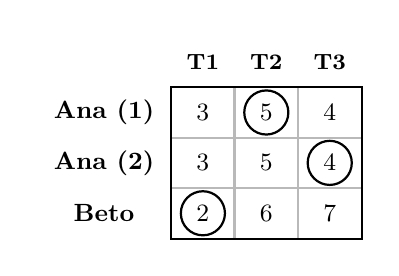
\begin{tikzpicture}
\matrix (c4) [mini, column 1/.style={nodes={text width=16mm, font=\small\bfseries}}] {
 \& T1 \& T2 \& T3 \\
Ana (1) \& 3 \& 5 \& 4 \\
Ana (2) \& 3 \& 5 \& 4 \\
Beto    \& 2 \& 6 \& 7 \\
};
\rejilla{c4}{4}{4}
\cero{c4}{2-3}\cero{c4}{3-4}\cero{c4}{4-2}
\end{tikzpicture}
\end{minipage}\hfill
\begin{minipage}[c]{0.62\textwidth}
\textit{Ejemplo:} Ana puede hacer dos tareas y Beto una. Se copia la fila de Ana y la tabla queda de $3 \times 3$.
El resultado (los círculos) es Ana $\to$ T2 y T3, Beto $\to$ T1, con costo $5 + 4 + 2 = 11$.
Al leer la respuesta se juntan las copias: ``Ana (1)'' y ``Ana (2)'' son la misma persona.
\end{minipage}

\paso{Caso 5. Óptimos múltiples: varias formas de escoger los ceros}
Al llegar al paso 5 puede pasar que haya \textbf{más de una forma} de escoger un cero por fila y por columna.
Como todos los ceros de la tabla final valen lo mismo (cero), \textbf{todas esas asignaciones cuestan lo mismo}:
son óptimos múltiples.

\begin{minipage}[c]{0.52\textwidth}
\centering
\begin{tikzpicture}
\matrix (c5) [mini] {
 \& T1 \& T2 \& T3 \\
Ana  \& 0 \& 0 \& 4 \\
Beto \& 0 \& 0 \& 1 \\
Caro \& 2 \& 5 \& 0 \\
};
\rejilla{c5}{4}{4}
\cero{c5}{2-2}\cero{c5}{3-3}\cero{c5}{4-4}
\pie{c5}{4}{4}{opción A}
\end{tikzpicture}\quad
\begin{tikzpicture}
\matrix (c5b) [mini] {
 \& T1 \& T2 \& T3 \\
Ana  \& 0 \& 0 \& 4 \\
Beto \& 0 \& 0 \& 1 \\
Caro \& 2 \& 5 \& 0 \\
};
\rejilla{c5b}{4}{4}
\cero{c5b}{2-3}\cero{c5b}{3-2}\cero{c5b}{4-4}
\pie{c5b}{4}{4}{opción B}
\end{tikzpicture}
\end{minipage}\hfill
\begin{minipage}[c]{0.46\textwidth}
\textit{Ejemplo:} en esta tabla final Ana y Beto tienen ceros en T1 y en T2. Se puede asignar Ana $\to$ T1 y
Beto $\to$ T2 (opción A) o al revés (opción B). Las dos cuestan lo mismo.
\end{minipage}

\medskip
Esto es una buena noticia para quien decide: puede elegir entre varias asignaciones igual de baratas usando otro
criterio (preferencias, experiencia, cercanía). Una advertencia: cuando las dos opciones solo \textbf{intercambian
copias del mismo agente} (caso 4), no son planes distintos en la realidad, solo nombres distintos para el mismo plan.
Esto ocurre en el ejercicio 3 de la Parte II.

\paso{Caso 6 (breve). Empates al tapar los ceros}
Si hay varias formas de tapar los ceros con el mínimo de líneas, o varios números empatados como menor sin tapar,
cualquier elección es válida y lleva al mismo costo mínimo. La calculadora siempre elige con la misma regla, y
este documento usa las mismas líneas que ella para que se puedan comparar paso a paso.

\needspace{14\baselineskip}
\begin{idea}[Resumen: cómo preparar la tabla]
\begin{enumerate}[leftmargin=*, itemsep=3pt]
  \item \textbf{¿Algún agente hace varias tareas?} Copiar su fila una vez por cada tarea que pueda hacer.
  \item \textbf{¿Es de maximizar?} Cambiar cada valor por $\text{mayor} - \text{valor}$.
  \item \textbf{¿Hay parejas prohibidas?} Poner $M$ en esas casillas.
  \item \textbf{¿La tabla no es cuadrada?} Agregar filas o columnas ficticias con 0.
  \item Resolver con el \textbf{método húngaro} (pasos 1 a 5).
  \item \textbf{Traducir:} juntar las copias, decir qué quedó sin pareja (lo ficticio) y sumar los
        \textbf{valores originales}. Si alguna pareja asignada tiene $M$, el problema es infactible.
\end{enumerate}
\end{idea}

\begin{center}
\begin{tikzpicture}[scale=0.74, transform shape, >=Stealth,
  caja/.style={draw, rounded corners=2pt, fill=gray!8, align=center, text width=2.6cm, inner sep=3pt, font=\small},
  decision/.style={draw, diamond, aspect=2.2, fill=gray!18, align=center, inner sep=1pt, font=\footnotesize},
  fin/.style={draw, rounded corners=8pt, fill=gray!25, align=center, inner sep=5pt, font=\small}]
  \foreach \k/\x/\t/\a in {1/0/{¿Un agente hace\\ varias tareas?}/{Duplicar su fila},
                           2/4.1/{¿Es de\\ maximizar?}/{Pérdida $=$ mayor $-$ valor},
                           3/8.2/{¿Hay parejas\\ prohibidas?}/{Poner $M$},
                           4/12.3/{¿La tabla no\\ es cuadrada?}/{Agregar ficticios con 0}} {
    \node[decision] (d\k) at (\x,0) {\t};
    \node[caja] (a\k) at (\x,-2.0) {\a};
    \draw[->] (d\k) -- node[right, font=\scriptsize] {sí} (a\k);
  }
  \foreach \k/\m in {1/2,2/3,3/4} {
    \draw[->] (d\k) -- node[above, font=\scriptsize] {no} (d\m);
    \draw[->] (a\k.east) -| ($(d\k.east)!0.5!(d\m.west)$);
  }
  \node[caja, fill=gray!25, font=\small\bfseries, text width=2.2cm] (h) at (16.1,0) {Método húngaro};
  \draw[->] (d4) -- node[above, font=\scriptsize] {no} (h);
  \draw[->] (a4.east) -| ($(d4.east)!0.5!(h.west)$);
  \node[decision] (d5) at (16.1,-3.6) {¿Quedó asignada\\ alguna $M$?};
  \draw[->] (h) -- (d5);
  \node[fin] (inf) at (12.3,-3.6) {\textbf{Infactible}};
  \node[fin] (ok) at (16.1,-5.4) {\textbf{Traducir el resultado}};
  \draw[->] (d5) -- node[above, font=\scriptsize] {sí} (inf);
  \draw[->] (d5) -- node[right, font=\scriptsize] {no} (ok);
\end{tikzpicture}
\end{center}

% =====================================================================
\section{¿Cómo se sabe que terminó?}

\begin{description}[leftmargin=0pt, itemsep=5pt]
  \item[Se puede asignar.] En el paso 3 hacen falta tantas líneas como filas tiene la tabla (ya cuadrada).
        Entonces existe un cero en cada fila y en cada columna sin repetir, y esa asignación es la óptima.
  \item[El resultado se lee en el problema real.] Se quitan las parejas ficticias, se juntan las copias y el total
        se calcula con los \textbf{valores originales}, no con la tabla final ni con la de pérdidas.
  \item[Problema infactible.] Si para asignar a todos hay que usar una casilla con $M$, no existe ninguna forma
        de repartir respetando las prohibiciones.
\end{description}

% =====================================================================
\section{Ventajas y desventajas}

\begin{center}\small
\begin{tabular}{p{7.2cm}p{7.2cm}}
\toprule
\textbf{Ventajas} & \textbf{Desventajas} \\
\midrule
\begin{itemize}[leftmargin=*, itemsep=2pt, topsep=2pt]
  \item Un solo método (el húngaro) resuelve todos los casos; solo cambia la preparación.
  \item Las transformaciones son restas y copias: se hacen a mano en minutos.
  \item Lo ficticio dice directamente qué tarea queda sin hacer o qué agente queda libre.
\end{itemize}
&
\begin{itemize}[leftmargin=*, itemsep=2pt, topsep=2pt]
  \item Duplicar filas y agregar ficticios agranda la tabla y alarga el trabajo.
  \item Con $M$ hay que llevar cuentas como $M - 870$, que se prestan a confusión.
  \item Si cada tarea se pudiera repartir entre varios agentes, ya no es asignación: es un problema de transporte.
\end{itemize}
\\
\bottomrule
\end{tabular}
\end{center}

\enlargethispage{3\baselineskip}
\textbf{Relación con la programación lineal.} Cada caso particular también se puede escribir como un programa
lineal con variables $x_{ij}$ ($= 1$ si el agente $i$ hace la tarea $j$). Lo no balanceado se vuelve
``$\le 1$'' en lugar de ``$= 1$'', la capacidad de un agente se vuelve ``$\le 2$'', y una pareja prohibida
simplemente no tiene variable. Así es como se comprobaron los ejercicios con el Simplex del primer previo.

% =====================================================================
\newpage
\part{Ejercicios resueltos}
\setcounter{section}{0}

Cada ejercicio muestra un caso particular distinto. Se sigue exactamente el mismo orden de pasos que la
calculadora: primero se prepara la tabla y luego se aplican los pasos del método húngaro de la
sección~\ref{sec:repaso}.

% =====================================================================
\section{Job Shop Co.: tres máquinas y cuatro ubicaciones}
\textit{Fuente: Hillier y Lieberman, Introducción a la Investigación de Operaciones, capítulo de los problemas
de transporte y asignación. Casos: no balanceado y asignación prohibida.}

\subsection*{Planteamiento del problema}
La compañía Job Shop compró \textbf{tres máquinas nuevas} de distinto tipo. En el taller hay \textbf{cuatro
ubicaciones} donde se puede instalar una máquina. Según lo cerca que quede cada máquina de los centros de trabajo,
cambia el \textbf{costo de mover los materiales}. La \textbf{ubicación 2 no sirve para la máquina 2} (no cabe).
Los costos estimados, en dólares por hora, son:

\begin{center}
\begin{tabular}{lcccc}
\toprule
 & \textbf{Ubicación 1} & \textbf{Ubicación 2} & \textbf{Ubicación 3} & \textbf{Ubicación 4} \\
\midrule
Máquina 1 & 13 & 16 & 12 & 11 \\
Máquina 2 & 15 & --- & 13 & 20 \\
Máquina 3 & 5 & 7 & 10 & 6 \\
\bottomrule
\end{tabular}
\end{center}

La pregunta: \textbf{¿en qué ubicación conviene instalar cada máquina para que el costo de manejo de materiales
sea el menor posible?}

\subsection*{Formulación del modelo}
\begin{itemize}[itemsep=2pt]
  \item Agentes: las 3 máquinas. Tareas: las 4 ubicaciones. Cada máquina va en una ubicación y en cada ubicación
        cabe a lo sumo una máquina.
  \item $x_{ij} = 1$ si la máquina $i$ se instala en la ubicación $j$, y 0 si no.
  \item Objetivo: $\text{Min } Z = 13x_{11} + 16x_{12} + 12x_{13} + 11x_{14} + 15x_{21} + 13x_{23} + 20x_{24} + 5x_{31} + 7x_{32} + 10x_{33} + 6x_{34}$.
  \item Cada máquina en una ubicación: $\sum_j x_{ij} = 1$. Cada ubicación con a lo sumo una máquina:
        $\sum_i x_{ij} \le 1$. La pareja (máquina 2, ubicación 2) no tiene variable.
\end{itemize}

\subsection*{Preparación de la tabla}
\begin{minipage}[c]{0.44\textwidth}
\begin{itemize}[itemsep=2pt, leftmargin=*]
  \item \textbf{No balanceado:} hay 3 máquinas y 4 ubicaciones. Se agrega una \textbf{máquina ficticia} con
        costo 0. La ubicación que le toque se quedará vacía.
  \item \textbf{Prohibida:} en la casilla (máquina 2, ubicación 2) se pone $M$.
\end{itemize}
\end{minipage}\hfill
\begin{minipage}[c]{0.54\textwidth}
\centering
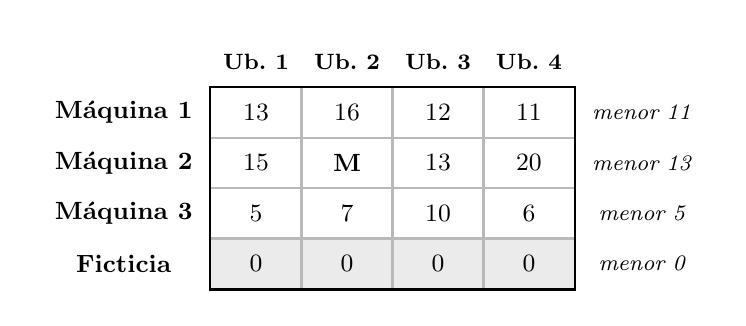
\begin{tikzpicture}
\matrix (a) [htab, nota col=6] {
 \& Ub.~1 \& Ub.~2 \& Ub.~3 \& Ub.~4 \& \\
Máquina 1 \& 13 \& 16 \& 12 \& 11 \& menor 11 \\
Máquina 2 \& 15 \& \cajaM \& 13 \& 20 \& menor 13 \\
Máquina 3 \& 5 \& 7 \& 10 \& 6 \& menor 5 \\
Ficticia  \& 0 \& 0 \& 0 \& 0 \& menor 0 \\
};
\sfila{a}{5}{5}
\rejilla{a}{5}{5}
\end{tikzpicture}
\end{minipage}

\medskip
Ahora la tabla es de $4 \times 4$: ya se puede usar el método húngaro.

\paso{Paso 1. Restar el menor de cada fila}
\begin{align*}
\text{Máquina 1:}&\ (13,\,16,\,12,\,11) - 11 = (2,\,5,\,1,\,0) \nota{el menor es 11}\\
\text{Máquina 2:}&\ (15,\,M,\,13,\,20) - 13 = (2,\,M-13,\,0,\,7) \nota{$M - 13$ sigue siendo gigantesco}\\
\text{Máquina 3:}&\ (5,\,7,\,10,\,6) - 5 = (0,\,2,\,5,\,1)\\
\text{Ficticia:}&\ (0,\,0,\,0,\,0) - 0 = (0,\,0,\,0,\,0) \nota{la fila ficticia ya es toda ceros}
\end{align*}

\paso{Paso 2. Restar el menor de cada columna}
Los menores de las columnas son $0,\ 0,\ 0,\ 0$: la fila ficticia pone un cero en cada columna, así que
\textbf{no cambia nada}. Esto pasa siempre que se agrega una fila ficticia.

\paso{Paso 3. Tapar los ceros con el menor número de líneas}
Hacen falta \textbf{4 líneas} (la calculadora tapa las cuatro filas). Como la tabla tiene 4 filas,
\textbf{ya se puede asignar}; no hace falta el paso 4.

\begin{center}
\begin{tikzpicture}
\matrix (b) [htab] {
 \& Ub.~1 \& Ub.~2 \& Ub.~3 \& Ub.~4 \\
Máquina 1 \& 2 \& 5 \& 1 \& 0 \\
Máquina 2 \& 2 \& $M{-}13$ \& 0 \& 7 \\
Máquina 3 \& 0 \& 2 \& 5 \& 1 \\
Ficticia  \& 0 \& 0 \& 0 \& 0 \\
};
\sfila{b}{5}{5}
\lfila{b}{2}{5}\lfila{b}{3}{5}\lfila{b}{4}{5}\lfila{b}{5}{5}
\rejilla{b}{5}{5}
\pie{b}{5}{5}{4 líneas $=$ 4 filas}
\end{tikzpicture}\qquad
\begin{tikzpicture}
\matrix (c) [htab] {
 \& Ub.~1 \& Ub.~2 \& Ub.~3 \& Ub.~4 \\
Máquina 1 \& 2 \& 5 \& 1 \& 0 \\
Máquina 2 \& 2 \& $M{-}13$ \& 0 \& 7 \\
Máquina 3 \& 0 \& 2 \& 5 \& 1 \\
Ficticia  \& 0 \& 0 \& 0 \& 0 \\
};
\sfila{c}{5}{5}
\rejilla{c}{5}{5}
\cero{c}{2-5}\cero{c}{3-4}\cero{c}{4-2}\cero{c}{5-3}
\pie{c}{5}{5}{asignación}
\end{tikzpicture}
\end{center}

\paso{Paso 5. Asignar un cero por fila y columna}
\begin{align*}
&1)\ \text{Máquina 1} \to \text{Ubicación 4} \nota{único cero de su fila: tacho su fila y su columna}\\
&2)\ \text{Máquina 2} \to \text{Ubicación 3} \nota{único cero de su fila}\\
&3)\ \text{Máquina 3} \to \text{Ubicación 1} \nota{único cero de su fila}\\
&4)\ \text{Ficticia} \to \text{Ubicación 2} \nota{es el único cero que queda libre}
\end{align*}

\subsection*{Resultado}
\[
\res{\text{M1} \to \text{Ub.~4},\quad \text{M2} \to \text{Ub.~3},\quad \text{M3} \to \text{Ub.~1},\quad Z^* = 29 \text{ dólares por hora}}
\]
\begin{itemize}[itemsep=2pt]
  \item La máquina 1 va en la ubicación 4 (\$11), la 2 en la ubicación 3 (\$13) y la 3 en la ubicación 1 (\$5).
  \item La \textbf{ubicación 2 queda vacía}: es la que le tocó a la máquina ficticia.
  \item El costo total de manejo de materiales es $11 + 13 + 5 = $ \textbf{\$29 por hora}.
\end{itemize}

\textbf{Comprobación:} cada máquina tiene una sola ubicación \checkmark; ninguna ubicación tiene dos máquinas
\checkmark; no se usó la pareja prohibida (máquina 2, ubicación 2) \checkmark; de las 24 formas de colocar las 3 máquinas,
18 respetan la prohibición, y entre ellas la más barata cuesta 29 y la siguiente 31 \checkmark.

\subsection*{Interpretación gráfica}
\begin{center}
\begin{tikzpicture}[>=Stealth, x=1cm, y=1.15cm]
  \foreach \i/\y in {1/3,2/2,3/1} \node[nodo, minimum size=8.5mm] (m\i) at (0,\y) {M\i};
  \node[nodo, minimum size=8.5mm, dashed, fill=gray!15] (mf) at (0,0) {F};
  \foreach \j/\y in {1/3,2/2,3/1,4/0} \node[nodo, minimum size=8.5mm] (u\j) at (5.5,\y) {U\j};
  \foreach \i in {1,2,3} \foreach \j in {1,2,3,4} \draw[gray!45] (m\i) -- (u\j);
  \draw[line width=2.2pt] (m1) -- node[etq, pos=0.13] {11} (u4);
  \draw[line width=2.2pt] (m2) -- node[etq, pos=0.13] {13} (u3);
  \draw[line width=2.2pt] (m3) -- node[etq, pos=0.13] {5} (u1);
  \draw[thick, dashed] (mf) -- node[etq, pos=0.13] {0} (u2);
  \draw[very thick, dotted] (m2) -- node[etq, pos=0.75] {\textbf{M}} (u2);
  \node[left=2mm of m1, font=\small] {Máquina 1};
  \node[left=2mm of m2, font=\small] {Máquina 2};
  \node[left=2mm of m3, font=\small] {Máquina 3};
  \node[left=2mm of mf, font=\small] {Ficticia};
  \node[right=2mm of u1, font=\small] {Ubicación 1};
  \node[right=2mm of u2, font=\small] {Ubicación 2 (vacía)};
  \node[right=2mm of u3, font=\small] {Ubicación 3};
  \node[right=2mm of u4, font=\small] {Ubicación 4};
\end{tikzpicture}
\end{center}
Las líneas gruesas son las parejas elegidas, con su costo por hora. La línea punteada con $M$ es la pareja
prohibida, y la discontinua es la ``pareja'' de la máquina ficticia. \textbf{En palabras:} aquí cada
máquina puede ir a su ubicación más barata (11, 13 y 5) sin chocar con las demás, y queda libre la ubicación 2,
que de todos modos no servía para la máquina 2. Así se gastan \$29 por hora en mover materiales, lo mínimo posible.

% =====================================================================
\section{Vendedores y zonas: maximizar las ventas}
\textit{Fuente: ejercicio adaptado (datos propios), en el estilo de los ejercicios de asignación de Taha y de
Anderson, Sweeney y Williams. Caso: maximización.}

\subsection*{Planteamiento del problema}
Una distribuidora tiene \textbf{cuatro vendedores} (Ana, Beto, Carla y Diego) y debe darle a cada uno
\textbf{una zona} de la ciudad (Norte, Sur, Este y Oeste). Por su experiencia y sus contactos, cada vendedor vende
distinto en cada zona. Las ventas esperadas, en miles de dólares por mes, son:

\begin{center}
\begin{tabular}{lcccc}
\toprule
 & \textbf{Norte} & \textbf{Sur} & \textbf{Este} & \textbf{Oeste} \\
\midrule
Ana   & 44 & 80 & 52 & 60 \\
Beto  & 60 & 56 & 40 & 72 \\
Carla & 36 & 60 & 48 & 48 \\
Diego & 52 & 76 & 36 & 40 \\
\bottomrule
\end{tabular}
\end{center}

La pregunta: \textbf{¿qué zona le toca a cada vendedor para que las ventas totales sean las más altas posibles?}

\subsection*{Formulación del modelo}
\begin{itemize}[itemsep=2pt]
  \item $x_{ij} = 1$ si el vendedor $i$ atiende la zona $j$, y 0 si no.
  \item Objetivo: $\text{Max } Z = 44x_{11} + 80x_{12} + 52x_{13} + 60x_{14} + \dots + 76x_{42} + 36x_{43} + 40x_{44}$.
  \item Cada vendedor en una zona y cada zona con un vendedor: $\sum_j x_{ij} = 1$, \ $\sum_i x_{ij} = 1$.
\end{itemize}
La tabla ya es cuadrada (4 vendedores y 4 zonas) y no hay prohibiciones. Lo único especial es que se busca el
\textbf{máximo}.

\subsection*{Preparación de la tabla: pérdida de oportunidad}
El mayor valor de la tabla es \textbf{80} (Ana en el Sur). Cada casilla se cambia por $80 - \text{valor}$
(por ejemplo $80 - 44 = 36$, \ $80 - 80 = 0$): lo que se deja de vender por elegir esa pareja en lugar de la mejor.
Así queda la tabla de la izquierda, con el menor de cada fila anotado al lado.

\begin{center}
\begin{tikzpicture}[baseline=(p-1-2.north)]
\matrix (p) [htab=9.2mm, nota col=6, column 1/.style={nodes={text width=13.5mm, font=\small\bfseries}}] {
 \& Norte \& Sur \& Este \& Oeste \& \\
Ana   \& 36 \& 0  \& 28 \& 20 \& menor 0 \\
Beto  \& 20 \& 24 \& 40 \& 8  \& menor 8 \\
Carla \& 44 \& 20 \& 32 \& 32 \& menor 20 \\
Diego \& 28 \& 4  \& 44 \& 40 \& menor 4 \\
};
\rejilla{p}{5}{5}
\pie{p}{5}{5}{$\text{pérdida} = 80 - \text{venta}$}
\end{tikzpicture}\qquad
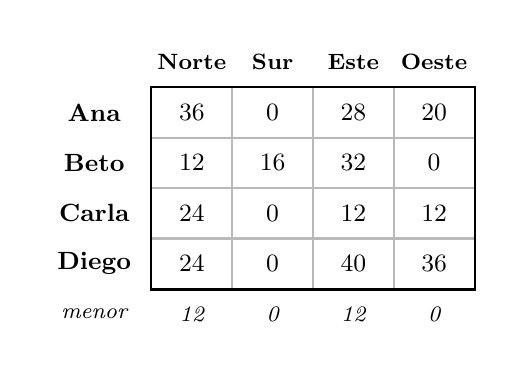
\begin{tikzpicture}[baseline=(p1-1-2.north)]
\matrix (p1) [htab=9.2mm, column 1/.style={nodes={text width=13.5mm, font=\small\bfseries}}] {
 \& Norte \& Sur \& Este \& Oeste \\
Ana   \& 36 \& 0  \& 28 \& 20 \\
Beto  \& 12 \& 16 \& 32 \& 0  \\
Carla \& 24 \& 0  \& 12 \& 12 \\
Diego \& 24 \& 0  \& 40 \& 36 \\
|[font=\footnotesize\itshape]| menor \& |[font=\footnotesize\itshape]| 12 \& |[font=\footnotesize\itshape]| 0 \& |[font=\footnotesize\itshape]| 12 \& |[font=\footnotesize\itshape]| 0 \\
};
\rejilla{p1}{5}{5}
\end{tikzpicture}
\end{center}

\paso{Paso 1. Restar el menor de cada fila}
A Ana se le resta 0 (ya tenía un cero), a Beto 8, a Carla 20 y a Diego 4. Por ejemplo, Beto:
$(20,\,24,\,40,\,8) - 8 = (12,\,16,\,32,\,0)$. Resultado: la tabla de la derecha.

\paso{Paso 2. Restar el menor de cada columna}
En la tabla de la derecha los menores de las columnas son Norte 12, Sur 0, Este 12 y Oeste 0. Se restan 12 en
Norte y 12 en Este, y se obtiene la tabla de abajo.

\begin{minipage}[c]{0.45\textwidth}
\centering
\begin{tikzpicture}
\matrix (q) [htab] {
 \& Norte \& Sur \& Este \& Oeste \\
Ana   \& 24 \& 0  \& 16 \& 20 \\
Beto  \& 0  \& 16 \& 20 \& 0  \\
Carla \& 12 \& 0  \& 0  \& 12 \\
Diego \& \textbf{12} \& 0  \& 28 \& 36 \\
};
\lfila{q}{3}{5}\lfila{q}{4}{5}\lcol{q}{3}{5}
\rejilla{q}{5}{5}
\pie{q}{5}{5}{3 líneas: filas Beto y Carla,\\ columna Sur}
\end{tikzpicture}
\end{minipage}\hfill
\begin{minipage}[c]{0.52\textwidth}
\paso{Paso 3. Tapar los ceros con el menor número de líneas}
Los ceros se tapan con \textbf{3 líneas}: la fila de Beto, la fila de Carla y la columna Sur.
Como $3 < 4$, \textbf{todavía no se puede asignar}: Ana y Diego solo tienen ceros en el Sur y los dos no pueden
ir a la misma zona. Hay que crear más ceros.
\end{minipage}

\paso{Paso 4. Ajustar con el menor número sin tapar}
Los números sin ninguna línea son los de Ana y Diego en Norte, Este y Oeste: $24, 16, 20, 12, 28, 36$.
El menor es
\[
k = 12 \nota{Diego en el Norte}
\]
\begin{itemize}[itemsep=2pt]
  \item A los números \textbf{sin tapar} se les resta 12: Ana queda $(12,\,\cdot,\,4,\,8)$ y Diego $(0,\,\cdot,\,16,\,24)$.
  \item A los \textbf{cruces de dos líneas} se les suma 12: Beto--Sur $16 + 12 = 28$ y Carla--Sur $0 + 12 = 12$.
  \item Lo que está tapado por una sola línea no cambia.
\end{itemize}

\paso{Paso 3 (otra vez). Tapar los ceros}
\begin{center}
\begin{tikzpicture}
\matrix (s) [htab] {
 \& Norte \& Sur \& Este \& Oeste \\
Ana   \& 12 \& 0  \& 4  \& 8  \\
Beto  \& 0  \& 28 \& 20 \& 0  \\
Carla \& 12 \& 12 \& 0  \& 12 \\
Diego \& 0  \& 0  \& 16 \& 24 \\
};
\lfila{s}{2}{5}\lfila{s}{3}{5}\lfila{s}{4}{5}\lfila{s}{5}{5}
\rejilla{s}{5}{5}
\pie{s}{5}{5}{4 líneas $=$ 4 filas}
\end{tikzpicture}\qquad
\begin{tikzpicture}
\matrix (t) [htab] {
 \& Norte \& Sur \& Este \& Oeste \\
Ana   \& 12 \& 0  \& 4  \& 8  \\
Beto  \& 0  \& 28 \& 20 \& 0  \\
Carla \& 12 \& 12 \& 0  \& 12 \\
Diego \& 0  \& 0  \& 16 \& 24 \\
};
\rejilla{t}{5}{5}
\cero{t}{2-3}\cero{t}{3-5}\cero{t}{4-4}\cero{t}{5-2}
\pie{t}{5}{5}{asignación}
\end{tikzpicture}
\end{center}
Ahora hacen falta \textbf{4 líneas} (una por fila), así que ya se puede asignar.

\paso{Paso 5. Asignar un cero por fila y columna}
\begin{align*}
&1)\ \text{Ana} \to \text{Sur} \nota{único cero de su fila: tacho la columna Sur}\\
&2)\ \text{Carla} \to \text{Este} \nota{único cero de su fila}\\
&3)\ \text{Diego} \to \text{Norte} \nota{su cero del Sur ya está tachado}\\
&4)\ \text{Beto} \to \text{Oeste} \nota{su cero del Norte ya está tachado}
\end{align*}

\subsection*{Resultado}
Las ventas se calculan con la \textbf{tabla original}, no con la de pérdidas:
\[
\res{\text{Ana} \to \text{Sur},\ \text{Beto} \to \text{Oeste},\ \text{Carla} \to \text{Este},\ \text{Diego} \to \text{Norte},\quad Z^* = 252}
\]
\begin{itemize}[itemsep=2pt]
  \item Ventas: $80 + 72 + 48 + 52 = 252$ mil dólares por mes, lo máximo posible.
  \item La pérdida total en la tabla de pérdidas es $0 + 8 + 32 + 28 = 68$, y en efecto $4 \cdot 80 - 68 = 252$.
\end{itemize}

\textbf{Comprobación:} cada vendedor tiene una zona y cada zona un vendedor \checkmark; las 24 formas posibles de
repartir dan como máximo 252, y la siguiente mejor da 244 \checkmark.

\subsection*{Interpretación gráfica}
\begin{minipage}[c]{0.50\textwidth}
\centering
\begin{tikzpicture}[>=Stealth]
  \foreach \n/\l/\y in {Ana/A/3,Beto/B/2,Carla/C/1,Diego/D/0} {\node[nodo] (\n) at (0,\y*0.95) {\l}; \node[left=2mm of \n, font=\small] {\n};}
  \foreach \n/\l/\y in {Norte/N/3,Sur/S/2,Este/E/1,Oeste/O/0} {\node[nodo] (\n) at (4.3,\y*0.95) {\l}; \node[right=2mm of \n, font=\small] {\n};}
  \foreach \a in {Ana,Beto,Carla,Diego} \foreach \z in {Norte,Sur,Este,Oeste} \draw[gray!40] (\a) -- (\z);
  \draw[line width=2.2pt] (Ana) -- node[etq, pos=0.25] {80} (Sur);
  \draw[line width=2.2pt] (Beto) -- node[etq, pos=0.25] {72} (Oeste);
  \draw[line width=2.2pt] (Carla) -- node[etq, pos=0.8] {48} (Este);
  \draw[line width=2.2pt] (Diego) -- node[etq, pos=0.15] {52} (Norte);
\end{tikzpicture}
\end{minipage}\hfill
\begin{minipage}[c]{0.47\textwidth}
\textbf{En palabras:} Ana se queda con el Sur, donde vende más que nadie (80). Diego también vendería mucho en el
Sur (76), pero como el Sur ya es de Ana, a Diego le conviene el Norte (52). Beto va al Oeste (72) y a Carla le toca
el Este (48). Fíjate en que \textbf{no basta con darle a cada uno su mejor zona}: Ana y Diego querrían el Sur, y el
método resuelve ese choque de la forma en que se pierden menos ventas.
\end{minipage}

% =====================================================================
\section{Better Products Co.: plantas que fabrican dos productos}
\textit{Fuente: Hillier y Lieberman, Introducción a la Investigación de Operaciones, capítulo de los problemas
de transporte y asignación. Casos: un agente con varias tareas, no balanceado, asignación prohibida y óptimos
múltiples aparentes.}

\subsection*{Planteamiento del problema}
La compañía Better Products va a empezar a fabricar \textbf{cuatro productos nuevos} en \textbf{tres plantas}
que tienen capacidad libre. Cada producto debe hacerse completo en una sola planta. Las plantas 1 y 2
\textbf{pueden encargarse de dos productos cada una}; la planta 3, de uno solo. Además, \textbf{la planta 2 no
puede fabricar el producto 3}. El costo de fabricar la producción diaria de cada producto en cada planta, en
dólares, es:

\begin{center}
\begin{tabular}{lccccc}
\toprule
 & \textbf{Producto 1} & \textbf{Producto 2} & \textbf{Producto 3} & \textbf{Producto 4} & \textbf{Capacidad} \\
\midrule
Planta 1 & 820 & 810 & 840 & 960 & 2 productos \\
Planta 2 & 800 & 870 & --- & 920 & 2 productos \\
Planta 3 & 740 & 900 & 810 & 840 & 1 producto \\
\bottomrule
\end{tabular}
\end{center}

La pregunta: \textbf{¿qué planta debe fabricar cada producto para que el costo diario total sea el menor?}

\subsection*{Formulación del modelo}
\begin{itemize}[itemsep=2pt]
  \item $x_{ij} = 1$ si la planta $i$ fabrica el producto $j$, y 0 si no.
  \item Objetivo: $\text{Min } Z = 820x_{11} + 810x_{12} + 840x_{13} + 960x_{14} + 800x_{21} + 870x_{22} + 920x_{24} + 740x_{31} + 900x_{32} + 810x_{33} + 840x_{34}$.
  \item Cada producto en una planta: $\sum_i x_{ij} = 1$.
  \item Capacidad de las plantas: $\sum_j x_{1j} \le 2$, \ $\sum_j x_{2j} \le 2$, \ $\sum_j x_{3j} \le 1$.
  \item La pareja (planta 2, producto 3) no tiene variable.
\end{itemize}

\subsection*{Preparación de la tabla}
\begin{minipage}[c]{0.44\textwidth}
\begin{itemize}[itemsep=2pt, leftmargin=*]
  \item \textbf{Varias tareas:} las plantas 1 y 2 pueden hacer dos productos, así que su fila se
        \textbf{copia}: Planta 1 (1), Planta 1 (2), Planta 2 (1), Planta 2 (2). Cada copia tiene los mismos costos.
  \item \textbf{No balanceado:} ahora hay 5 filas y solo 4 productos. Se agrega una \textbf{columna ficticia}
        con costo 0. La fila que la reciba es un ``turno'' de planta que no se usa.
  \item \textbf{Prohibida:} en las dos copias de la planta 2, la casilla del producto 3 vale $M$.
\end{itemize}
\end{minipage}\hfill
\begin{minipage}[c]{0.54\textwidth}
\centering
\resizebox{\linewidth}{!}{%
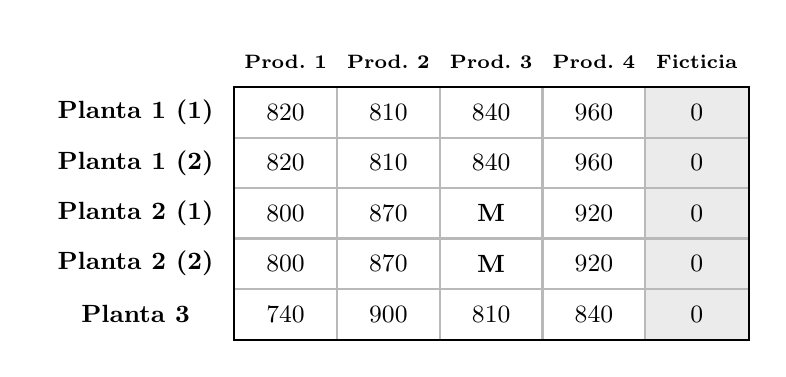
\begin{tikzpicture}
\matrix (x) [tab9] {
 \& Prod.~1 \& Prod.~2 \& Prod.~3 \& Prod.~4 \& Ficticia \\
Planta 1 (1) \& 820 \& 810 \& 840 \& 960 \& 0 \\
Planta 1 (2) \& 820 \& 810 \& 840 \& 960 \& 0 \\
Planta 2 (1) \& 800 \& 870 \& \cajaM \& 920 \& 0 \\
Planta 2 (2) \& 800 \& 870 \& \cajaM \& 920 \& 0 \\
Planta 3 \& 740 \& 900 \& 810 \& 840 \& 0 \\
};
\scol{x}{6}{6}
\rejilla{x}{6}{6}
\end{tikzpicture}}
\end{minipage}

\medskip
La tabla queda de $5 \times 5$.

\paso{Paso 1. Restar el menor de cada fila}
Todas las filas tienen un 0 en la columna ficticia, así que el menor de cada fila es 0 y \textbf{no cambia nada}.
Esto pasa siempre que se agrega una columna ficticia.

\paso{Paso 2. Restar el menor de cada columna}
Los menores de las columnas son 740 (producto 1, planta 3), 810 (producto 2, planta 1), 810 (producto 3,
planta 3), 840 (producto 4, planta 3) y 0 (ficticia). Al restar: $820 - 740 = 80$, \ $870 - 810 = 60$,
\ $M - 810$ (sigue gigantesco), etc. El resultado es la tabla de la izquierda:

\begin{center}
\resizebox{0.49\textwidth}{!}{%
\begin{tikzpicture}
\matrix (y) [tab9] {
 \& Prod.~1 \& Prod.~2 \& Prod.~3 \& Prod.~4 \& Ficticia \\
Planta 1 (1) \& 80 \& 0 \& 30 \& 120 \& 0 \\
Planta 1 (2) \& 80 \& 0 \& 30 \& 120 \& 0 \\
Planta 2 (1) \& 60 \& 60 \& $M{-}810$ \& 80 \& 0 \\
Planta 2 (2) \& 60 \& 60 \& $M{-}810$ \& 80 \& 0 \\
Planta 3 \& 0 \& 90 \& 0 \& 0 \& 0 \\
};
\scol{y}{6}{6}
\lfila{y}{6}{6}\lcol{y}{3}{6}\lcol{y}{6}{6}
\rejilla{y}{6}{6}
\pie{y}{6}{6}{después del paso 2: 3 líneas}
\end{tikzpicture}
}\hfill
\resizebox{0.49\textwidth}{!}{%
\begin{tikzpicture}
\matrix (z) [tab9] {
 \& Prod.~1 \& Prod.~2 \& Prod.~3 \& Prod.~4 \& Ficticia \\
Planta 1 (1) \& 50 \& 0 \& 0 \& 90 \& 0 \\
Planta 1 (2) \& 50 \& 0 \& 0 \& 90 \& 0 \\
Planta 2 (1) \& 30 \& 60 \& $M{-}840$ \& 50 \& 0 \\
Planta 2 (2) \& 30 \& 60 \& $M{-}840$ \& 50 \& 0 \\
Planta 3 \& 0 \& 120 \& 0 \& 0 \& 30 \\
};
\scol{z}{6}{6}
\lfila{z}{2}{6}\lfila{z}{3}{6}\lfila{z}{6}{6}\lcol{z}{6}{6}
\rejilla{z}{6}{6}
\pie{z}{6}{6}{después del primer ajuste: 4 líneas}
\end{tikzpicture}
}
\end{center}

\paso{Paso 3. Tapar los ceros}
Bastan \textbf{3 líneas}: la fila de la planta 3, la columna del producto 2 y la columna ficticia (tabla de la
izquierda). Como $3 < 5$, todavía no se puede asignar.

\paso{Paso 4. Primer ajuste}
Los números sin tapar están en las filas de las plantas 1 y 2, columnas de los productos 1, 3 y 4:
$80, 30, 120, 60, M - 810, 80$. El menor es
\[
k = 30 \nota{planta 1, producto 3}
\]
Se resta 30 a lo no tapado (por ejemplo $80 \to 50$, $60 \to 30$, $M - 810 \to M - 840$) y se suma 30 en los
cruces: planta 3--producto 2 ($90 \to 120$) y planta 3--ficticia ($0 \to 30$). Queda la tabla de la derecha.

\paso{Paso 3 (otra vez). Tapar los ceros}
Ahora hacen falta \textbf{4 líneas}: las filas de la planta 1 (las dos copias), la fila de la planta 3 y la
columna ficticia. Como $4 < 5$, hay que ajustar otra vez.

\paso{Paso 4. Segundo ajuste}
Lo único sin tapar son las dos filas de la planta 2 en los productos 1 a 4: $30, 60, M - 840, 50$. El menor es
\[
k = 30 \nota{planta 2, producto 1}
\]
Se resta 30 en esas casillas ($30 \to 0$, $60 \to 30$, $M - 840 \to M - 870$, $50 \to 20$) y se suma 30 en los
cruces de la columna ficticia con las filas tapadas: las dos copias de la planta 1 ($0 \to 30$) y la planta 3
($30 \to 60$).

\paso{Paso 3 (otra vez). Tapar los ceros}
Ahora hacen falta \textbf{5 líneas} (la calculadora tapa las cinco filas), así que ya se puede asignar.

\begin{center}
\resizebox{0.49\textwidth}{!}{%
\begin{tikzpicture}
\matrix (w) [tab9] {
 \& Prod.~1 \& Prod.~2 \& Prod.~3 \& Prod.~4 \& Ficticia \\
Planta 1 (1) \& 50 \& 0 \& 0 \& 90 \& 30 \\
Planta 1 (2) \& 50 \& 0 \& 0 \& 90 \& 30 \\
Planta 2 (1) \& 0 \& 30 \& $M{-}870$ \& 20 \& 0 \\
Planta 2 (2) \& 0 \& 30 \& $M{-}870$ \& 20 \& 0 \\
Planta 3 \& 0 \& 120 \& 0 \& 0 \& 60 \\
};
\scol{w}{6}{6}
\rejilla{w}{6}{6}
\cero{w}{2-3}\cero{w}{3-4}\cero{w}{4-2}\cero{w}{5-6}\cero{w}{6-5}
\pie{w}{6}{6}{asignación de la calculadora}
\end{tikzpicture}
}\hfill
\resizebox{0.49\textwidth}{!}{%
\begin{tikzpicture}
\matrix (v) [tab9] {
 \& Prod.~1 \& Prod.~2 \& Prod.~3 \& Prod.~4 \& Ficticia \\
Planta 1 (1) \& 50 \& 0 \& 0 \& 90 \& 30 \\
Planta 1 (2) \& 50 \& 0 \& 0 \& 90 \& 30 \\
Planta 2 (1) \& 0 \& 30 \& $M{-}870$ \& 20 \& 0 \\
Planta 2 (2) \& 0 \& 30 \& $M{-}870$ \& 20 \& 0 \\
Planta 3 \& 0 \& 120 \& 0 \& 0 \& 60 \\
};
\scol{v}{6}{6}
\rejilla{v}{6}{6}
\cero{v}{2-4}\cero{v}{3-3}\cero{v}{4-6}\cero{v}{5-2}\cero{v}{6-5}
\pie{v}{6}{6}{otra asignación con el mismo total}
\end{tikzpicture}
}
\end{center}

\needspace{8\baselineskip}
\paso{Paso 5. Asignar un cero por fila y columna}
\begin{align*}
&1)\ \text{Planta 3} \to \text{Prod. 4} \nota{único cero de la columna del producto 4}\\
&2)\ \text{Planta 1 (1)} \to \text{Prod. 2} \nota{había dos ceros: elijo uno}\\
&3)\ \text{Planta 1 (2)} \to \text{Prod. 3} \nota{único cero libre de su fila}\\
&4)\ \text{Planta 2 (1)} \to \text{Prod. 1} \nota{había dos ceros: elijo uno}\\
&5)\ \text{Planta 2 (2)} \to \text{Ficticia} \nota{único cero libre de su fila}
\end{align*}

\subsection*{Resultado}
\[
\res{\text{P1} \to \text{Prod. 2 y 3},\quad \text{P2} \to \text{Prod. 1},\quad \text{P3} \to \text{Prod. 4},\quad Z^* = 3\,290 \text{ dólares por día}}
\]
\begin{itemize}[itemsep=2pt]
  \item La planta 1 fabrica los productos 2 y 3 ($810 + 840$), la planta 2 el producto 1 ($800$) y la planta 3 el
        producto 4 ($840$). Costo diario total: $810 + 840 + 800 + 840 = $ \textbf{\$3\,290}.
  \item La copia Planta 2 (2) quedó con la columna ficticia: la planta 2 \textbf{usa solo uno} de sus dos turnos.
\end{itemize}

\subsection*{Óptimos múltiples}
En la tabla final \textbf{hay otra forma de escoger los ceros} con el mismo total: es la tabla de la derecha que aparece antes del paso 5.
Planta 1 (1) $\to$ Prod. 3, Planta 1 (2) $\to$ Prod. 2, Planta 2 (1) $\to$ Ficticia, Planta 2 (2) $\to$ Prod. 1 y
Planta 3 $\to$ Prod. 4. También suma $840 + 810 + 800 + 840 = 3\,290$.

Pero fíjate bien: lo único que cambió es \textbf{cuál copia} de la planta 1 hace cada producto y \textbf{cuál copia}
de la planta 2 queda libre. En la fábrica real el plan es el mismo: la planta 1 hace los productos 2 y 3, la planta 2
el producto 1 y la planta 3 el producto 4. Es el aviso del caso 5: cuando se duplican filas, los óptimos múltiples
pueden ser solo ``el mismo plan con otros nombres''. Por eso la calculadora \textbf{no} lo anuncia como óptimo
múltiple: solo avisa cuando cambia alguna pareja real planta--producto. Revisando todas las formas reales de repartir
los productos, este plan es el único que cuesta 3\,290; el siguiente cuesta 3\,310.

\textbf{Comprobación:} cada producto tiene una sola planta \checkmark; la planta 1 hace 2 productos
($\le 2$) \checkmark, la planta 2 hace 1 ($\le 2$) \checkmark{} y la planta 3 hace 1 ($\le 1$) \checkmark; la planta 2 no
fabrica el producto 3 \checkmark.

\subsection*{Interpretación gráfica}
\begin{minipage}[c]{0.56\textwidth}
\centering
\begin{tikzpicture}[>=Stealth, scale=0.85]
  \foreach \i/\y in {1/3,2/1.5,3/0} \node[nodo, minimum size=9mm] (p\i) at (0,\y) {P\i};
  \foreach \j/\y in {1/3.3,2/2.2,3/1.1,4/0} \node[nodo, minimum size=8mm] (r\j) at (5,\y) {\j};
  \foreach \i in {1,2,3} \foreach \j in {1,2,3,4} \draw[gray!40] (p\i) -- (r\j);
  \draw[very thick, dotted] (p2) -- node[etq, pos=0.55] {\textbf{M}} (r3);
  \draw[line width=2.2pt] (p1) -- node[etq, pos=0.7] {810} (r2);
  \draw[line width=2.2pt] (p1) -- node[etq, pos=0.7] {840} (r3);
  \draw[line width=2.2pt] (p2) -- node[etq, pos=0.2] {800} (r1);
  \draw[line width=2.2pt] (p3) -- node[etq, pos=0.35] {840} (r4);
  \node[left=2mm of p1, font=\small, align=right] {Planta 1\\ \footnotesize hace 2 de 2};
  \node[left=2mm of p2, font=\small, align=right] {Planta 2\\ \footnotesize hace 1 de 2};
  \node[left=2mm of p3, font=\small, align=right] {Planta 3\\ \footnotesize hace 1 de 1};
  \foreach \j in {1,2,3,4} \node[right=1mm of r\j, font=\small] {Prod.~\j};
\end{tikzpicture}
\end{minipage}\hfill
\begin{minipage}[c]{0.41\textwidth}
\textbf{En palabras:} la planta 3 es la más barata para casi todo, pero solo puede hacer un producto; se le da el
producto 4, donde las otras plantas son mucho más caras (960 y 920). La planta 1 se encarga de los productos 2 y 3
y la planta 2, que no puede hacer el producto 3, se queda con el producto 1. A la planta 2 le sobra capacidad para
un producto más. El costo diario es de \$3\,290.
\end{minipage}

% =====================================================================
\section*{Resumen de los tres ejercicios}
\begin{center}\small
\begin{tabular}{>{\raggedright\arraybackslash}p{2.2cm}>{\raggedright\arraybackslash}p{4.0cm}>{\raggedright\arraybackslash}p{1.9cm}>{\raggedright\arraybackslash}p{4.0cm}c}
\toprule
\textbf{Ejercicio} & \textbf{Casos particulares} & \textbf{Tabla} & \textbf{Asignación} & \textbf{Óptimo} \\
\midrule
Job Shop Co. & no balanceado (fila ficticia), prohibida ($M$) & $4 \times 4$, 0 ajustes & M1--Ub.~4, M2--Ub.~3, M3--Ub.~1; Ub.~2 vacía & \$29/h \\
Vendedores y zonas & maximización (pérdida de oportunidad) & $4 \times 4$, 1 ajuste & Ana--Sur, Beto--Oeste, Carla--Este, Diego--Norte & 252 mil \\
Better Products & varias tareas (filas copiadas), no balanceado (columna ficticia), prohibida, óptimo múltiple aparente & $5 \times 5$, 2 ajustes & P1--Prod.~2 y 3, P2--Prod.~1, P3--Prod.~4 & \$3\,290/día \\
\bottomrule
\end{tabular}
\end{center}

\begin{idea}[Conclusiones]
\begin{itemize}[itemsep=0pt, leftmargin=*]
  \item Los casos particulares \textbf{no necesitan otro método}: se prepara la tabla y se usa el húngaro de siempre.
  \item \textbf{No balanceado:} filas o columnas ficticias con 0. Lo asignado a lo ficticio queda sin pareja.
  \item \textbf{Maximización:} se resta cada valor del mayor y se minimiza la pérdida; el total se suma con los valores originales.
  \item \textbf{Prohibidas:} costo $M$. Si el método se ve obligado a usar una $M$, el problema es infactible.
  \item \textbf{Varias tareas:} se copia la fila del agente; al final se juntan las copias.
  \item \textbf{Óptimos múltiples:} si hay otra forma de escoger los ceros, cuesta lo mismo; pero si solo cambia
        qué copia hace qué, es el mismo plan.
\end{itemize}
\end{idea}

\textbf{Verificación:} los tres ejercicios se resolvieron con la calculadora (\emph{Simplex Arcade}, modo
Asignación, memorias 7, 8 y 9), que muestra los mismos pasos, líneas, valores de $k$ y asignaciones de este documento.
Además, cada uno se planteó como programa lineal y se resolvió con el Simplex de la calculadora y con la librería
javascript-lp-solver, y se revisaron por fuerza bruta todas las asignaciones posibles. Los tres métodos coinciden:
29, 252 y 3\,290.

\section*{Referencias}
\addcontentsline{toc}{part}{Referencias}
\begin{itemize}[leftmargin=*, itemsep=1pt]\small
  \item Anderson, D. R., Sweeney, D. J. y Williams, T. A. \textit{Métodos cuantitativos para los negocios}. Cengage Learning. Capítulo de modelos de distribución y de redes (problema de asignación).
  \item Hillier, F. S. y Lieberman, G. J. \textit{Introducción a la Investigación de Operaciones}. McGraw-Hill. Capítulo de los problemas de transporte y asignación.
  \item Kuhn, H. W. (1955). The Hungarian method for the assignment problem. \textit{Naval Research Logistics Quarterly}, 2(1--2).
  \item Taha, H. A. \textit{Investigación de Operaciones}. Pearson. Capítulo del modelo de transporte y sus variantes (modelo de asignación).
  \item Winston, W. L. \textit{Investigación de Operaciones: aplicaciones y algoritmos}. Thomson. Capítulo de transporte, asignación y transbordo.
\end{itemize}

\end{document}
